
\providecommand{\weburl}{\url{https://leandojo.org}}
\providecommand{\name}{ReProver}
\providecommand{\numproofs}{98,734}
\providecommand{\numpremises}{130,262}
\providecommand{\numaccessiblepremises}{33,160}
\providecommand{\numtraintheorems}{94,734}
\providecommand{\numvaltheorems}{2,000}
\providecommand{\numtesttheorems}{2,000}
\providecommand{\numfiles}{3,384}
\providecommand{\numtactics}{217,776}
\providecommand{\numtacticswithpremises}{129,243}
\providecommand{\avgnumpremises}{2.13}
\definecolor{mygreen}{RGB}{226,240,217}
\definecolor{myblue}{RGB}{222,235,247}
\definecolor{myorange}{RGB}{251,229,214}
\definecolor{mygray}{RGB}{219,219,219}
\providecommand{\hlgreen}[1]{\colorbox{mygreen}{#1}}
\providecommand{\hlblue}[1]{\colorbox{myblue}{#1}}
\providecommand{\hlorange}[1]{\colorbox{myorange}{#1}}
\providecommand{\hlgray}[1]{\colorbox{mygray}{#1}}


\subsection*{Source Note}
This section is derived from LeanDojo, where Alex contributed but is not first
author. It is marked in blue in the thesis draft. The section includes only the
field-shaping material needed for this chapter: the evaluation object, the
benchmark design, and the way the environment made later system building
possible.

\subsection{Why LeanDojo Belongs in This Chapter}
LeanDojo is an example of measurement shaping what the field builds. Before a
community can reliably improve language-model theorem provers, it needs a
reproducible way to extract theorem-proving data, interact with the proof
assistant, and compare systems on a shared benchmark. LeanDojo provided that
infrastructure for Lean theorem proving.

The key shift is from isolated proof-generation examples to a programmable
evaluation loop. A theorem prover is not merely asked to emit a proof string.
It observes a Lean proof state, proposes a tactic, receives the next state or an
error, and repeats until the theorem is solved or the search fails. This turns
formal theorem proving into a measurable interactive task, where success is
checked by Lean itself.

\begin{figure}[tbp]
  \centering
  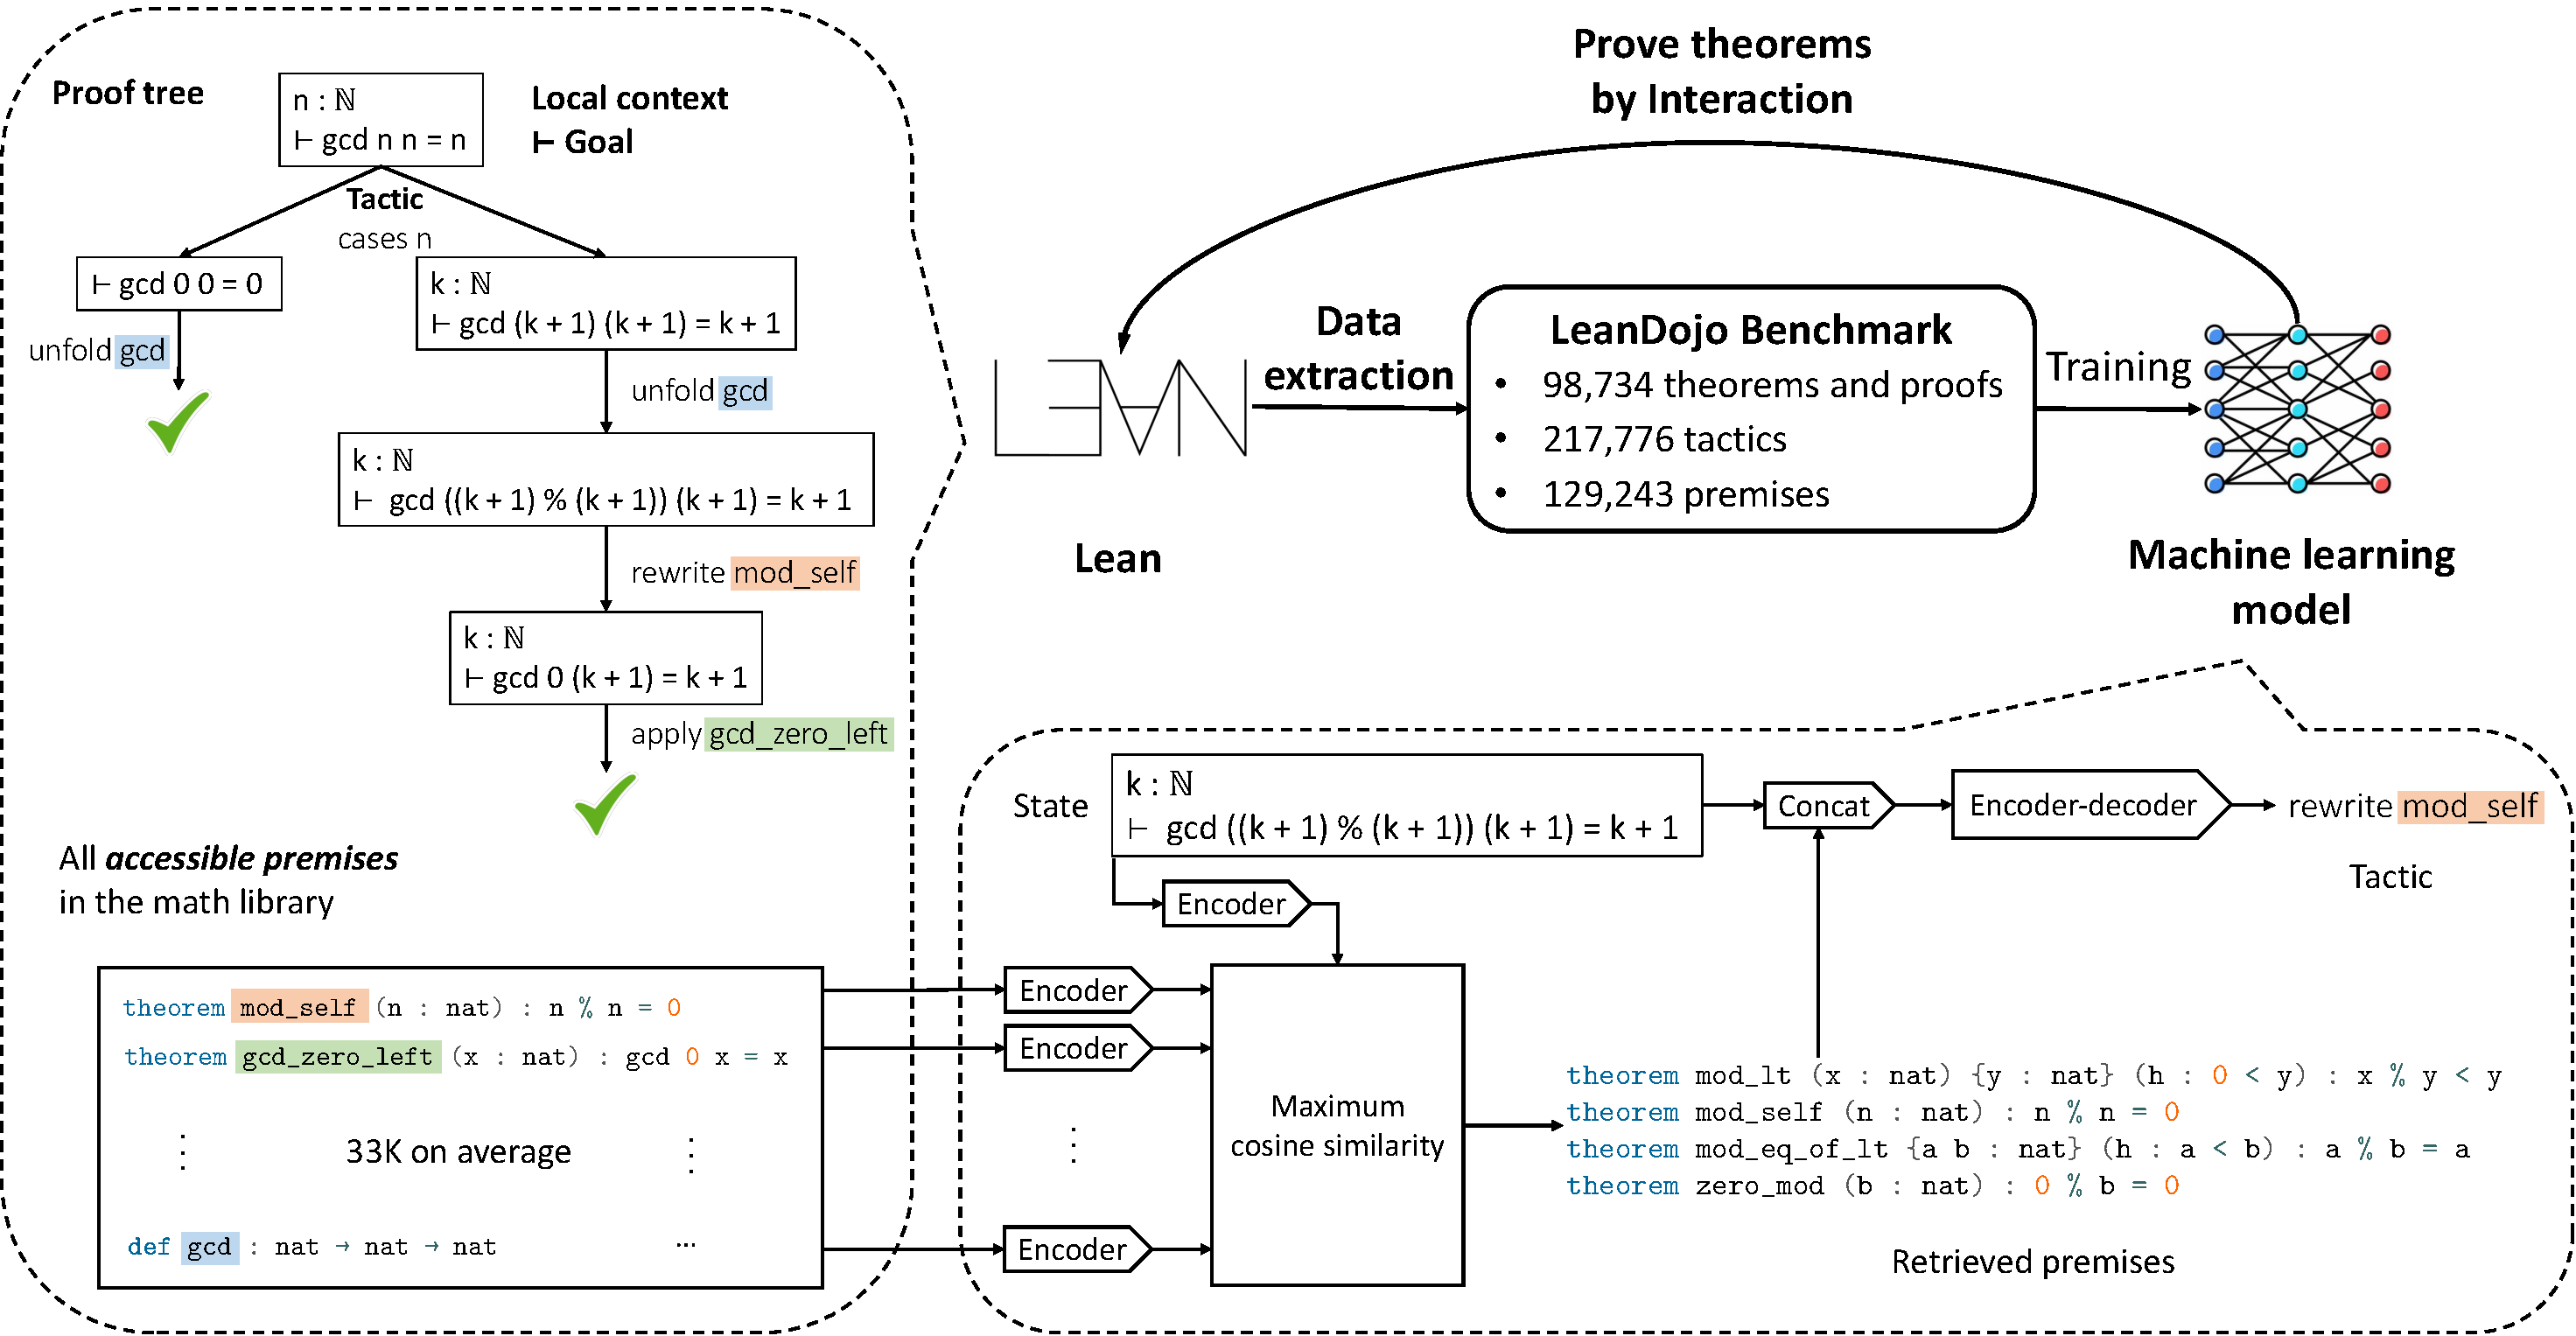
\includegraphics[width=0.95\linewidth]{figures/overall.pdf}
  \caption{LeanDojo connects data extraction, proof-state interaction, premise
  retrieval, and tactic generation into a reproducible theorem-proving
  environment.}
  \label{fig:leandojo-overall-thesis}
\end{figure}

\subsection{The Evaluation Object: Interaction With a Proof Assistant}
In Lean, proofs are built by applying tactics to proof states. Each tactic
transforms the current goals into simpler goals, fails with an error, or closes
the proof. Learning-based theorem proving therefore needs access to information
that is not visible from the raw source file alone: intermediate proof states,
tactics, file dependencies, abstract syntax trees, and the premises used by
proof steps.

LeanDojo extracts this information from Lean repositories and exposes a
programmatic interaction interface. A prover can initialize a theorem, observe
the current proof state, run a tactic, and receive feedback from Lean. This
interface makes the proof assistant part of the evaluation, not merely a
post-hoc checker. It also makes theorem proving a natural target for search,
retrieval, and reinforcement learning methods, because the model can receive
state-level feedback as it constructs a proof.

Reliability is part of the measurement contribution. If a correct proof is
misjudged as incorrect because the environment is constructed incorrectly, then
the benchmark underestimates the system. LeanDojo was designed to reduce this
kind of proof-checking error and to make Lean interaction reliable enough for
repeated model evaluation.

\subsection{Benchmark Design: Avoiding Memorized Near-Duplicates}
LeanDojo Benchmark was built from Lean's mathematical library and contains
\numproofs{} theorems/proofs from \numfiles{} files, together with information
about \numpremises{} premises and \numtactics{} tactics. The scale matters
because theorem proving systems need enough data for training and enough held
out tasks for meaningful evaluation.

The more important measurement decision is the split. Random theorem splits can
overestimate model ability because formal libraries often contain families of
nearly identical theorems with nearly identical proofs. If one theorem in such a
family appears in training and another appears in testing, a model can appear
to prove a difficult theorem by memorizing a proof pattern. LeanDojo therefore
introduced a more challenging \texttt{novel\_premises} split, where test proofs
require at least one premise that was not used in training proofs.

\begin{figure}[tbp]
  \centering
  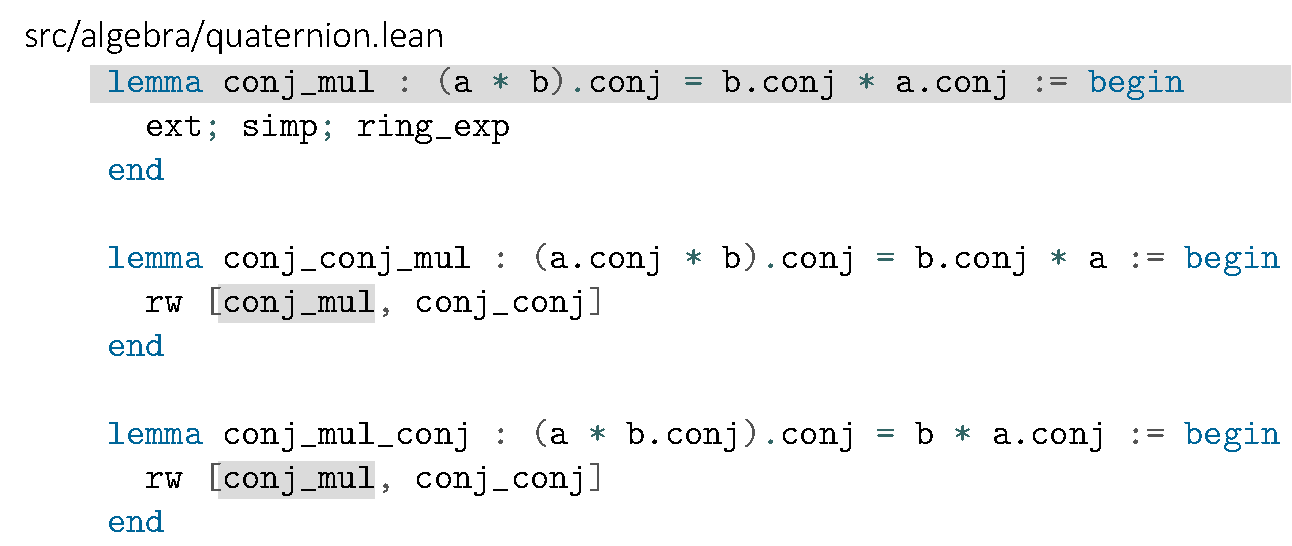
\includegraphics[width=0.72\linewidth]{figures/quaternion.pdf}
  \caption{Lean libraries contain clusters of similar theorems and proofs.
  Benchmark splits must account for this or they risk measuring memorization.}
  \label{fig:leandojo-quaternion-thesis}
\end{figure}

This connects directly to the thesis theme. The benchmark's structure changes
the claim we can make. A random split asks whether the model can solve held-out
theorems drawn from a distribution that may include close proof analogues. The
\texttt{novel\_premises} split asks whether the model can generalize to proofs
that require new library dependencies. Those are different measurements, and
they push system builders toward different capabilities.

\subsection{Retrieval as a System-Building Consequence}
LeanDojo also made premise selection a central engineering target. Large formal
libraries contain far more premises than can fit into a model context, but many
proofs depend on selecting the right definitions or lemmas. LeanDojo records
which premises are accessible and which are used, enabling retrieval-augmented
theorem proving rather than forcing models to memorize premise names.

The ReProver model built on this infrastructure retrieves relevant premises
from the library and conditions tactic generation on the proof state plus those
premises. This is a concrete example of measurement shaping what gets built.
Once the benchmark exposes premise selection and proof-state interaction as
measurable bottlenecks, the natural system design becomes retrieval plus tactic
generation, evaluated inside the Lean environment.

\subsection{Results and Field Effect}
On LeanDojo Benchmark, ReProver outperformed baselines that generated tactics
without retrieval and baselines that used GPT-4 in a zero-shot tactic-generation
setting. The results also showed that the \texttt{novel\_premises} split is
substantially harder than the random split, supporting the paper's claim that
random splits can inflate estimates of theorem-proving ability.

The broader effect is that LeanDojo gave the community a reusable evaluation
harness, dataset, and baseline model. Later theorem-proving work could use the
environment to train models, evaluate provers, retrieve premises, and interact
with Lean under a common protocol. In the terms of this chapter, LeanDojo did
not merely report a score; it helped define the target that future systems
would optimize.

\subsection{Thesis Takeaway}
LeanDojo shows how an evaluation can create a field-facing abstraction. By
making proof-assistant interaction reproducible, benchmarked, and accessible,
it changed theorem proving from a collection of hard-to-compare demonstrations
into a shared engineering problem. That is why it belongs in the chapter on how
measurement shapes what gets built.
